\section{Практычны занятак №1}

\subsection{Структура праекта}

На малюнку \ref{img: pz1} прадстаўлена файлавая структура праекта.

\begin{figure}[h!]
    \centering
    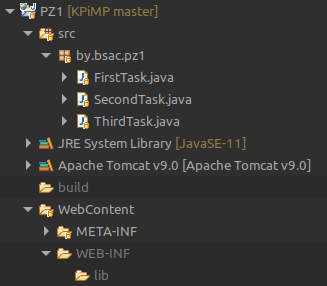
\includegraphics[width=0.5\textwidth]{pz1_structure}
    \caption{Файлавая структура практычнага занятку}
    \label{img: pz1} 
\end{figure}

\vspace{-\baselineskip}
\subsection{Заданне 1}

\subsubsection{Апісанне задання.}

Напісаць сервлет, які выдае HTML-старонка з полем для ўводу з
імем \textit{P1}. Перад полем для ўвода мусіць быць тэкст
\textit{Поля для ўвода:}.

\subsubsection{Зыходны код.}

Зыходны код з тлумачэннямі прадстаўлены
ў лістынгку \ref{lst: pz1_task1}.
\lstinputlisting[caption={Зыходны код для першага задання},%
                 label={lst: pz1_task1},%
                 language=Java]{PZ1/FirstTask.java}

\vspace{-\baselineskip}
\subsection{Заданне 2}

\subsubsection{Апісанне задання.}

Напісаць сервлет, які выдае HTML-старонку з полем для ўводу з імем
\textit{P1} і кнопкай \textit{Submit}. Пасля запаўнення карыстальнікам
поля для ўводу і націскання кнопкі \textit{Submit} сервлет мае выдаць
такую ж HTML-старонку, у полі \textit{P1} якога мае змяшчацца
ўведзенае значэнне, паўторанае 2 разы.

\subsubsection{Зыходны код.}

Зыходны код з тлумачэннямі прадстаўлены
ў лістынку \ref{lst: pz1_task2}.

\lstinputlisting[caption={Зыходны код для першага задання},%
                 label={lst: pz1_task2},%
                 language=Java]{PZ1/SecondTask.java}

\vspace{-\baselineskip}
\subsection{Заданне 3}

\subsubsection{Апісанне задання.}

Напісаць сервлет, які выдае HTML-старонку з лікам \textit{1} і
кнопкай \textit{Submit}. Пасля націскання кнопкі \textit{Submit}
сервлет павінен выдаць HTML-старонку з лікам \textit{2} і кнопкай
\textit{Submit}. Пасля з лікам \textit{3} і гэтак далей.

\subsubsection{Зыходны код.}

Зыходны код з тлумачэннямі прадстаўлены
ў лістынку \ref{lst: pz1_task3}.

\lstinputlisting[caption={Зыходны код для першага задання},%
                 label={lst: pz1_task3},%
                 language=Java]{PZ1/ThirdTask.java}
